\section{Implementation}\label{Sec_Imp}

\subsection{Communication (Abdul and/or Stefan)}

\subsection{Initialization procedure (Stephan and Stefan)}\label{Sec_Imp_Ini}

\subsubsection{Recording and filtering data (Stefan)}

\subsubsection{Analysing data (Stefan)}

\subsubsection[Selection of correct distance related to RSSI]{Selection of correct distance related to RSSI footnote{Stephan}}
In a first step the multiple occurring data points (see tbl.\ref{RSSI_Dis_data}) are divided into three groups (max, middle and min) where max means the maximal possible distance related to one RSSI and so on.\\ 
The measurements has shown that it is not trivial to define the correct distance related to most of the RSSI. The involved algorithm selects the correct distance out of the multiple possible solutions and is shown in fig. \ref{BestID}:\\
\begin{figure}[!htbp]
\centering
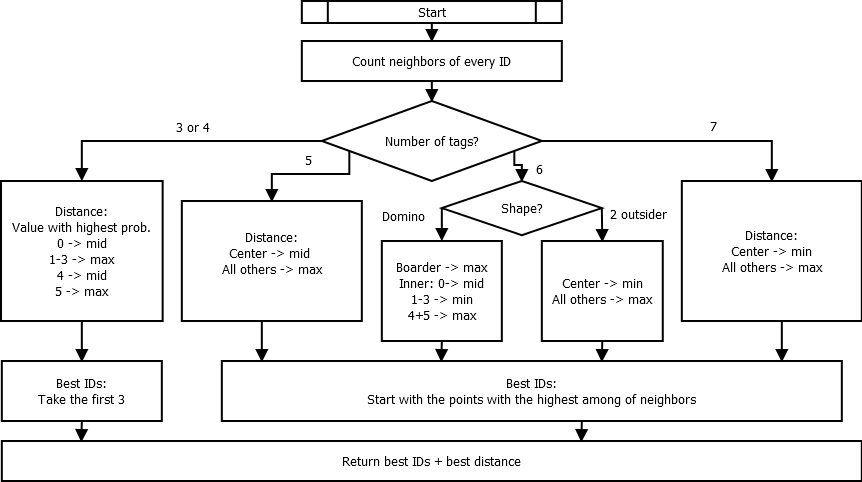
\includegraphics[width = 16cm]{Pictures/BestIDs}
\caption{Flow Chart: Selection of correct distance and most proper IDs}
\label{BestID}
\end{figure}\\
To distinguish between the multiple possible solution for one RSSI, the algorithm defines the shape of the pattern of tags based on the number of tags at each measurement and the number of the neighbours each tag has. At each measurement point are in this scenario several numbers (4-7) of detected tags possible. The different shapes can be found in the tbl. \ref{ID_shapes}.\\
\begin{table}[!htbp]
\centering
\begin{tabular}{|c|c|c|c|c|c|}
\hline
\begin{tabular}[c]{@{}c@{}}Number of \\ detected tags \end{tabular}  & 4 & 5 & 6 (Domino) & 6 (2 alone)& 7 \\ \hline
Unique shapes        & 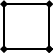
\includegraphics[width = 1.3cm]{Pictures/Shape1} & 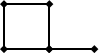
\includegraphics[width = 2.6cm]{Pictures/Shape2} &   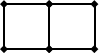
\includegraphics[width = 2.6cm]{Pictures/Shape3} & 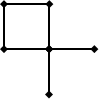
\includegraphics[width = 2.6cm]{Pictures/Shape4} & 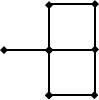
\includegraphics[width = 2.6cm]{Pictures/Shape5}\\ \hline
\end{tabular}
\caption{Possible shapes of pattern}
\label{ID_shapes}
\end{table}\\
Going back to the flow chart fig.\ref{BestID} the first step is to count the number of neighbours each tag has. With this information, the position of the tag in the pattern can be detected. For example is a tag with 3 neighbours in a pattern of 5 tags the center of this pattern.\\
After the number of tags at each measurement point and the position of each tag are defined, the selection of the correct distance will be performed based on the highest probability. To know the highest probabilities an analysis of measurements with emulated data has been done.\\
As an example are leading 4 detected tags to the fact that the position of the antenna should be very close to the center of this square. If in this case a RSSI of 4 is detected, the middle value (5.8 cm) will be taken. \\
Afterwards the most suitable three IDs will be selected, in case where more then three are detected. The algorithm takes at first the ID with the highest amount of neighbours, because these tags are close to the position of the antenna and have probably a value of 6 or 7 and are uniquely defined. In the case where several tags with the same number of neighbours, the first ID (number increasing) will be taken. \\
The return of the function is an array (2x3) with the indices of the chosen IDs and the correct distance. The correct distance will be indicated by the number 0,1 and 2. 0 means the maximal, 1 the middle and 2 the minimum possible value related to one RSSI. For example leads 
\[
\begin{bmatrix}
    3 & 2 & 4\\
    2 & 0 & 0 
\end{bmatrix} 
\]
to the choice of the maximal value of the RSSI of the fourth detected ID and the minimum value of the RSSI of the third and the fifth ID in the recorded array at this measurement point. \\

\subsubsection[Estimation of initial position and orientation]{Estimation of initial position and orientation \footnote{Stephan}}
As mentioned in chapter \ref{Sec_Imp_Ini}, the main idea to estimate the initial position is to find the intersection point, which lies in the middle of the measurement points.\\
To compute this position, the algorithm uses trilateration at every suitable measurement point to estimate its position. For trilatertion are three defined positions plus three radii necessary, which are available after the selection of the correct distance and proper IDs.\\
\begin{figure}[!htbp]
\centering
\begin{minipage}{.5\textwidth}
\centering
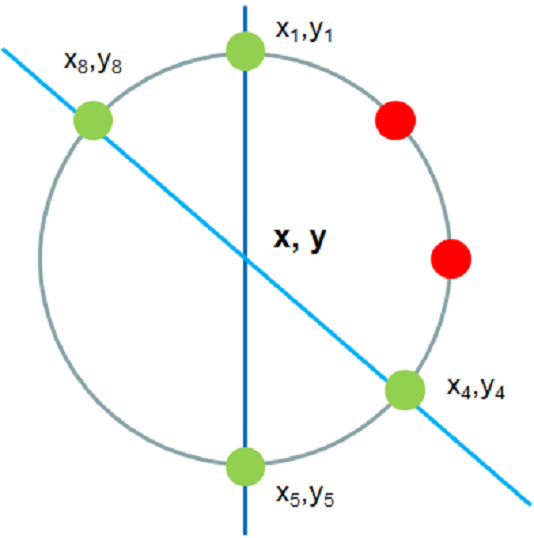
\includegraphics[width=5.5cm]{Pictures/Center_Rob} %
\caption{Computing the center of the robot}
\label{Center}
\end{minipage}%
\begin{minipage}{.5\textwidth}
\centering
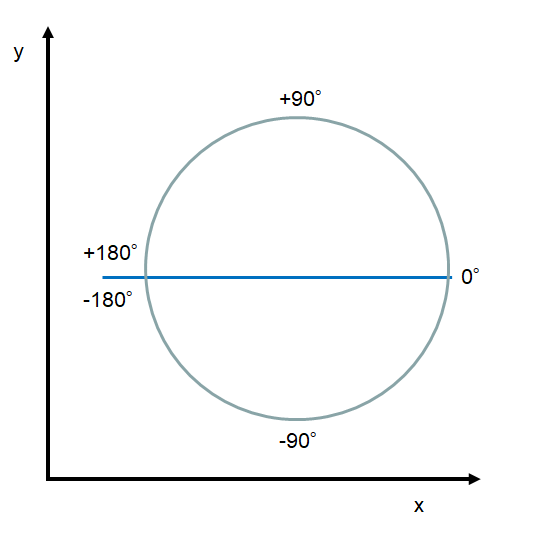
\includegraphics[width=5.5cm]{Pictures/Orientation} %
\caption{Orientation of robot in absolute angle}
\label{Angle}
\end{minipage}
\end{figure}\\
As follows from the fig.\ref{Center} shown above, the intersection point is found by computing two linear functions which go trough two corresponding points (blue lines). The center of the robot is then the intersection of those two linear functions and can be computed by the following equation:
\begin{align}
x = \dfrac{(x_1y_2-y_1x_2)(x_3-x_4)-(x_1-x_2)(x_3y_4-y_3x_4)}{(x_1-x_2)(y_3-y_4)-(y_1-y_2)(x_3-x_4)} \\
y = \dfrac{(x_1y_2-y_1x_2)(y_3-y_4)-(y_1-y_2)(x_3y_4-y_3x_4)}{(x_1-x_2)(y_3-y_4)-(y_1-y_2)(x_3-x_4)}
\end{align}
Theoretical are all eight measuring points suitable points (at least four IDs found). But for the case that the real measurements differ from the theory, the algorithm just needs four suitable points. \\
After the initial position as well as the positions of 4 measurement points are known, the algorithm computes the orientation based on those information. The relative angle between the center and the first measurement point will be computed with the arctan2 function and leads to an orientation -180$^\circ < \Theta \leq$180$^\circ$ as shown in fig.\ref{Angle}. \\
To compute the absolute angle, the angle of the measurement point has to be subtracted and 180$^\circ$ has to be added. This is caused by the fact that the antenna is placed on the back of the robot and the absolute orientation should be the direction of the front. After this computation, the initial position and orientation of the robot are known. \\

\subsection[Test setup]{Test setup\footnote{Stephan}}
In order to verify the validity of the initialization procedure, we carried out experiments with the components mentioned in chapter \ref{Sec_Har}. The beginning of these experiments were the reconstruction of one of the AGVs with this HW setup. After we added all components to the AGV we realized the power supply via a powerbank and the USB connection of then wifi modul. The plan is to replace this in the future with a direct connection to the battery of the AGV. Fig.\ref{TestSetup} gives an overview of the test setup and shows also that for the prototype, the reader and the wifi modul was just stuck with Sellotape on the upper layer of the AGV.\\
\begin{figure}[!htbp]
\centering
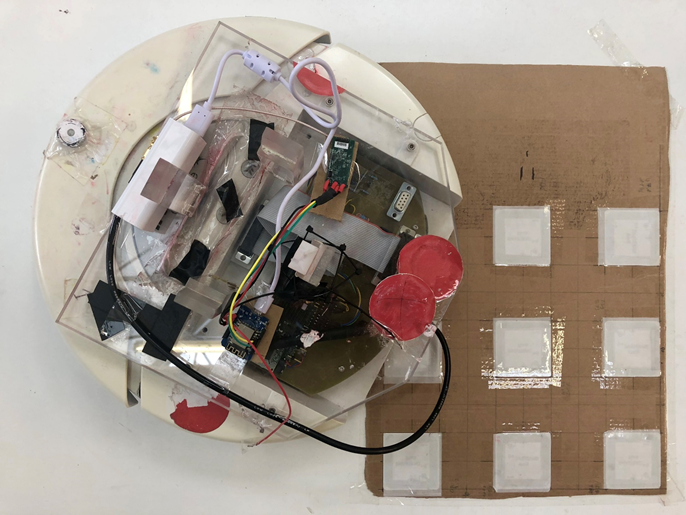
\includegraphics[width = 14cm]{Pictures/TestSetup}
\caption{testing setup for initialization procedure}
\label{TestSetup}
\end{figure}\\
The test platform was a field of 9 tags which were stuck on a piece of carton. The IDs and its positions are shown in tbl.\ref{IDs_Setup}.\\
\begin{table}[!htbp]
\begin{tabular}{|c|c|c|c|c|c|c|c|c|c|}
\hline
X-dir. [mm] & 0    & 100  & 200  & 0    & 100  & 200  & 0    & 100  & 200  \\ \hline
Y-dir. [mm] & 0    & 0    & 0    & 100  & 100  & 100  & 200  & 200  & 200  \\ \hline
ID tag [hex]    & AE4  & 689  & 47A  & 586  & 785  & ADC  & BF4  & 691  & 78D  \\ \hline
ID tag [dec]    & 2788 & 1673 & 1146 & 1414 & 1925 & 2780 & 3060 & 1681 & 1933 \\ \hline
\end{tabular}
\caption{Positions of the IDs in the test setup}
\label{IDs_Setup}
\end{table}\\
The reason for the small setup was the fact that until the end of the project only 10 tags were available. One of the following steps should be to extend the platform with more tags.\\
The initialization procedure was started via the GUI. A time value was added in the GUI to perform the 45$^\circ$ turns. This number was \textcolor{red}{around 1150 ms} and is highly correlated to the battery status of the AGV.\\

\subsection[Results]{Results\footnote{Stephan}}
A couple of tests on the test setup (previous section) were performed to compare the good results created with the simulated data with real measurements. The result of the position estimation was directly plotted in the console. The initial position was 200 mm in x- and y-direction and a varying orientation (0$^\circ$, 90$^\circ$, 180$^\circ$ and -90$^\circ$). Fig.\ref{ResultX} and fig.\ref{ResultY} illustrate the actual measurement results and the desired position in x- and y-direction. 
\begin{figure}[!htbp]
\centering
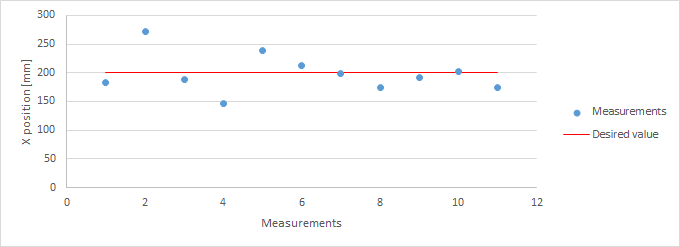
\includegraphics[width = 14cm]{Pictures/ResultX}
\caption{Estimated position in x-direction}
\label{ResultX}
\end{figure}\\
The average of the absolute error of the position in x-direction was 24.5 mm. The minimum and maximum error were 2 mm and 72 mm.\\
\begin{figure}[!htbp]
\centering
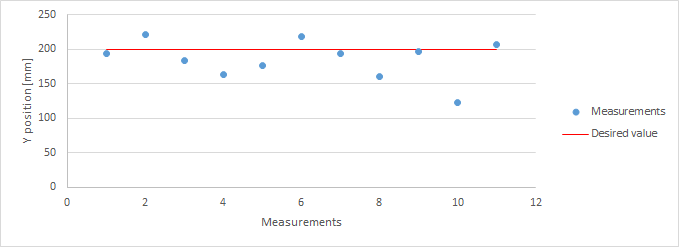
\includegraphics[width = 14cm]{Pictures/ResultY}
\caption{Estimated position in y-direction}
\label{ResultY}
\end{figure}\\
The average of the absolute error of the estimation of the position in y-direction is with 23.3 mm, a minimum error of 3 mm and an maximum error of 77 mm very similar to the results from the estimation of the x-direction. The computation of the overall error of the position has an average derivation of 37.5 mm and a minimum and maximum error of 6.3 mm and 77 mm.\\
\begin{figure}[!htbp]
\centering
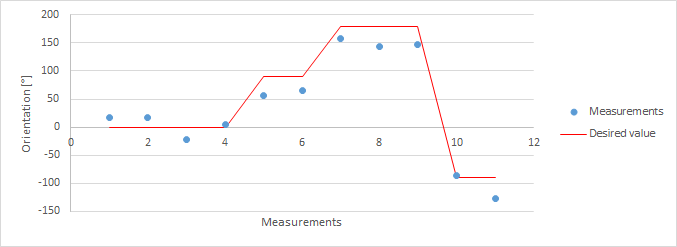
\includegraphics[width = 14cm]{Pictures/ResultO}
\caption{Estimated orientation}
\label{ResultO}
\end{figure}\\
For the estimation of the orientation, the average of the absolute error was 23$^\circ$ with a minimum and a maximum value of 3.9$^\circ$ and 37.5$^\circ$. The measurements also shows that an estimation of the position with a big error not necessarily leads to a big error in the estimation of the orientation (see measurement 4 in fig.\ref{ResultX},\ref{ResultY} and \ref{ResultO}).\\
An extension of the results could also be an analyse of the estimated positions of the antenna at the measurement points. Those points were also plotted in the console. \\

%\subsection{Improvements}

